\documentclass[tikz]{standalone}
\usepackage{tikz}
\usetikzlibrary{intersections,calc,quotes,angles}
\usepackage{tkz-euclide}
\begin{document}

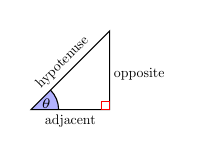
\begin{tikzpicture}
  \coordinate [] (A) at (0,0);
  \coordinate [] (B) at (1,1);
  \coordinate [] (C) at (1,0);
  
  \draw pic[draw,fill=blue!30,angle radius=10,"$\theta$",font=\tiny] {angle=C--A--B};    
  \draw (C) node[scale = .25,label={[scale=.5,xshift=.75cm,yshift=.3cm,label distance=.25cm]90:opposite}] {} -- (A) node[scale = .5,midway,sloped,anchor=north] {adjacent} -- (B)node[scale = .5,midway,sloped,above] {hypotenuse} -- cycle;
  \draw[red] (.9,0) rectangle ++(.1,.1);
  %\draw (1,0) arc[start angle=0, end angle=360, radius=1];
  %\draw pic[draw,fill=blue!30,angle radius=10,"$\theta$",font=\tiny] {};    
  %\draw (-1,0) -- (1,0);
  %\draw (0,-1) -- (0,1);
  %\draw (0,0) -- (.866025403784,.5) node[sloped, above right,scale = .5] {$\frac{\pi}{6}$};
  %\draw (0,0) -- (.707106781187,.707106781187) node[sloped, above right,scale = .5] {$\frac{\pi}{4}$};
  %\draw (0,0) -- (.5,.866025403784) node[sloped, above right,scale = .5] {$\frac{\pi}{3}$};
  %\draw (0,0) -- (0,1) node[sloped, above,scale = .5] {$\frac{\pi}{2}$};
  %\draw (0,0) -- (-.5,.866025403784) node[sloped, above left,scale = .5] {$\frac{2\pi}{3}$};
  %\draw (0,0) -- (-.707106781187,.707106781187) node[sloped, above left,scale = .5] {$\frac{3\pi}{4}$};
  %\draw (0,0) -- (-.866025403784,.5) node[sloped, above left,scale = .5] {$\frac{5\pi}{6}$};
  %\draw (0,0) -- (-1,0) node[sloped, left,scale = .5] {$\pi$};
  %
  %\draw (0,0) -- (-.866025403784,-.5) node[sloped, below left,scale = .5] {$\frac{7\pi}{6}$};
  %\draw (0,0) -- (-.707106781187,-.707106781187) node[sloped, below left,scale = .5] {$\frac{5\pi}{4}$};
  %\draw (0,0) -- (-.5,-.866025403784) node[sloped, below left,scale = .5] {$\frac{4\pi}{3}$};
  %\draw (0,0) -- (0,-1) node[sloped, below,scale = .5] {$\frac{3\pi}{2}$};
  %\draw (0,0) -- (.5,-.866025403784) node[sloped, below right,scale = .5] {$\frac{5\pi}{3}$};
  %\draw (0,0) -- (.707106781187,-.707106781187) node[sloped, below right,scale = .5] {$\frac{7\pi}{4}$};
  %\draw (0,0) -- (.866025403784,-.5) node[sloped, below right,scale = .5] {$\frac{11\pi}{6}$};
  %\draw (0,0) -- (1,0) node[sloped, right,scale = .5] {$0$ or $2\pi$};

\end{tikzpicture}
\end{document}